\documentclass[tikz,border=10pt]{standalone}
% Shared look for every TikZ diagram. Load with % Shared look for every TikZ diagram. Load with % Shared look for every TikZ diagram. Load with \input{../../tools/tikz-style.tex}
\usepackage[T1]{fontenc}
\usepackage{lmodern}
\renewcommand{\sfdefault}{lmr}  % diagrams use the same serif as the text
\usetikzlibrary{arrows.meta, positioning, shapes.geometric, calc, fit, backgrounds}
\definecolor{cblue}{HTML}{4C78A8}
\definecolor{corange}{HTML}{F58518}
\definecolor{cgreen}{HTML}{54A24B}
\definecolor{cred}{HTML}{E45756}
\definecolor{cpurple}{HTML}{B279A2}
\definecolor{cgrey}{HTML}{6B6B6B}
\tikzset{
  every picture/.style={font=\sffamily, line width=1.2pt},
  box/.style={draw=#1, fill=#1!12, rounded corners=4pt, align=center, inner sep=7pt, minimum height=1.1cm},
  box/.default=cgrey,
  arrow/.style={-{Stealth[length=3mm]}, draw=cgrey, line width=1.4pt},
  title/.style={font=\sffamily\bfseries\Large},
  note/.style={font=\sffamily\small, text=cgrey, align=center},
}
\AtBeginDocument{\hyphenpenalty=10000 \exhyphenpenalty=10000}

\usepackage[T1]{fontenc}
\usepackage{lmodern}
\renewcommand{\sfdefault}{lmr}  % diagrams use the same serif as the text
\usetikzlibrary{arrows.meta, positioning, shapes.geometric, calc, fit, backgrounds}
\definecolor{cblue}{HTML}{4C78A8}
\definecolor{corange}{HTML}{F58518}
\definecolor{cgreen}{HTML}{54A24B}
\definecolor{cred}{HTML}{E45756}
\definecolor{cpurple}{HTML}{B279A2}
\definecolor{cgrey}{HTML}{6B6B6B}
\tikzset{
  every picture/.style={font=\sffamily, line width=1.2pt},
  box/.style={draw=#1, fill=#1!12, rounded corners=4pt, align=center, inner sep=7pt, minimum height=1.1cm},
  box/.default=cgrey,
  arrow/.style={-{Stealth[length=3mm]}, draw=cgrey, line width=1.4pt},
  title/.style={font=\sffamily\bfseries\Large},
  note/.style={font=\sffamily\small, text=cgrey, align=center},
}
\AtBeginDocument{\hyphenpenalty=10000 \exhyphenpenalty=10000}

\usepackage[T1]{fontenc}
\usepackage{lmodern}
\renewcommand{\sfdefault}{lmr}  % diagrams use the same serif as the text
\usetikzlibrary{arrows.meta, positioning, shapes.geometric, calc, fit, backgrounds}
\definecolor{cblue}{HTML}{4C78A8}
\definecolor{corange}{HTML}{F58518}
\definecolor{cgreen}{HTML}{54A24B}
\definecolor{cred}{HTML}{E45756}
\definecolor{cpurple}{HTML}{B279A2}
\definecolor{cgrey}{HTML}{6B6B6B}
\tikzset{
  every picture/.style={font=\sffamily, line width=1.2pt},
  box/.style={draw=#1, fill=#1!12, rounded corners=4pt, align=center, inner sep=7pt, minimum height=1.1cm},
  box/.default=cgrey,
  arrow/.style={-{Stealth[length=3mm]}, draw=cgrey, line width=1.4pt},
  title/.style={font=\sffamily\bfseries\Large},
  note/.style={font=\sffamily\small, text=cgrey, align=center},
}
\AtBeginDocument{\hyphenpenalty=10000 \exhyphenpenalty=10000}

\begin{document}
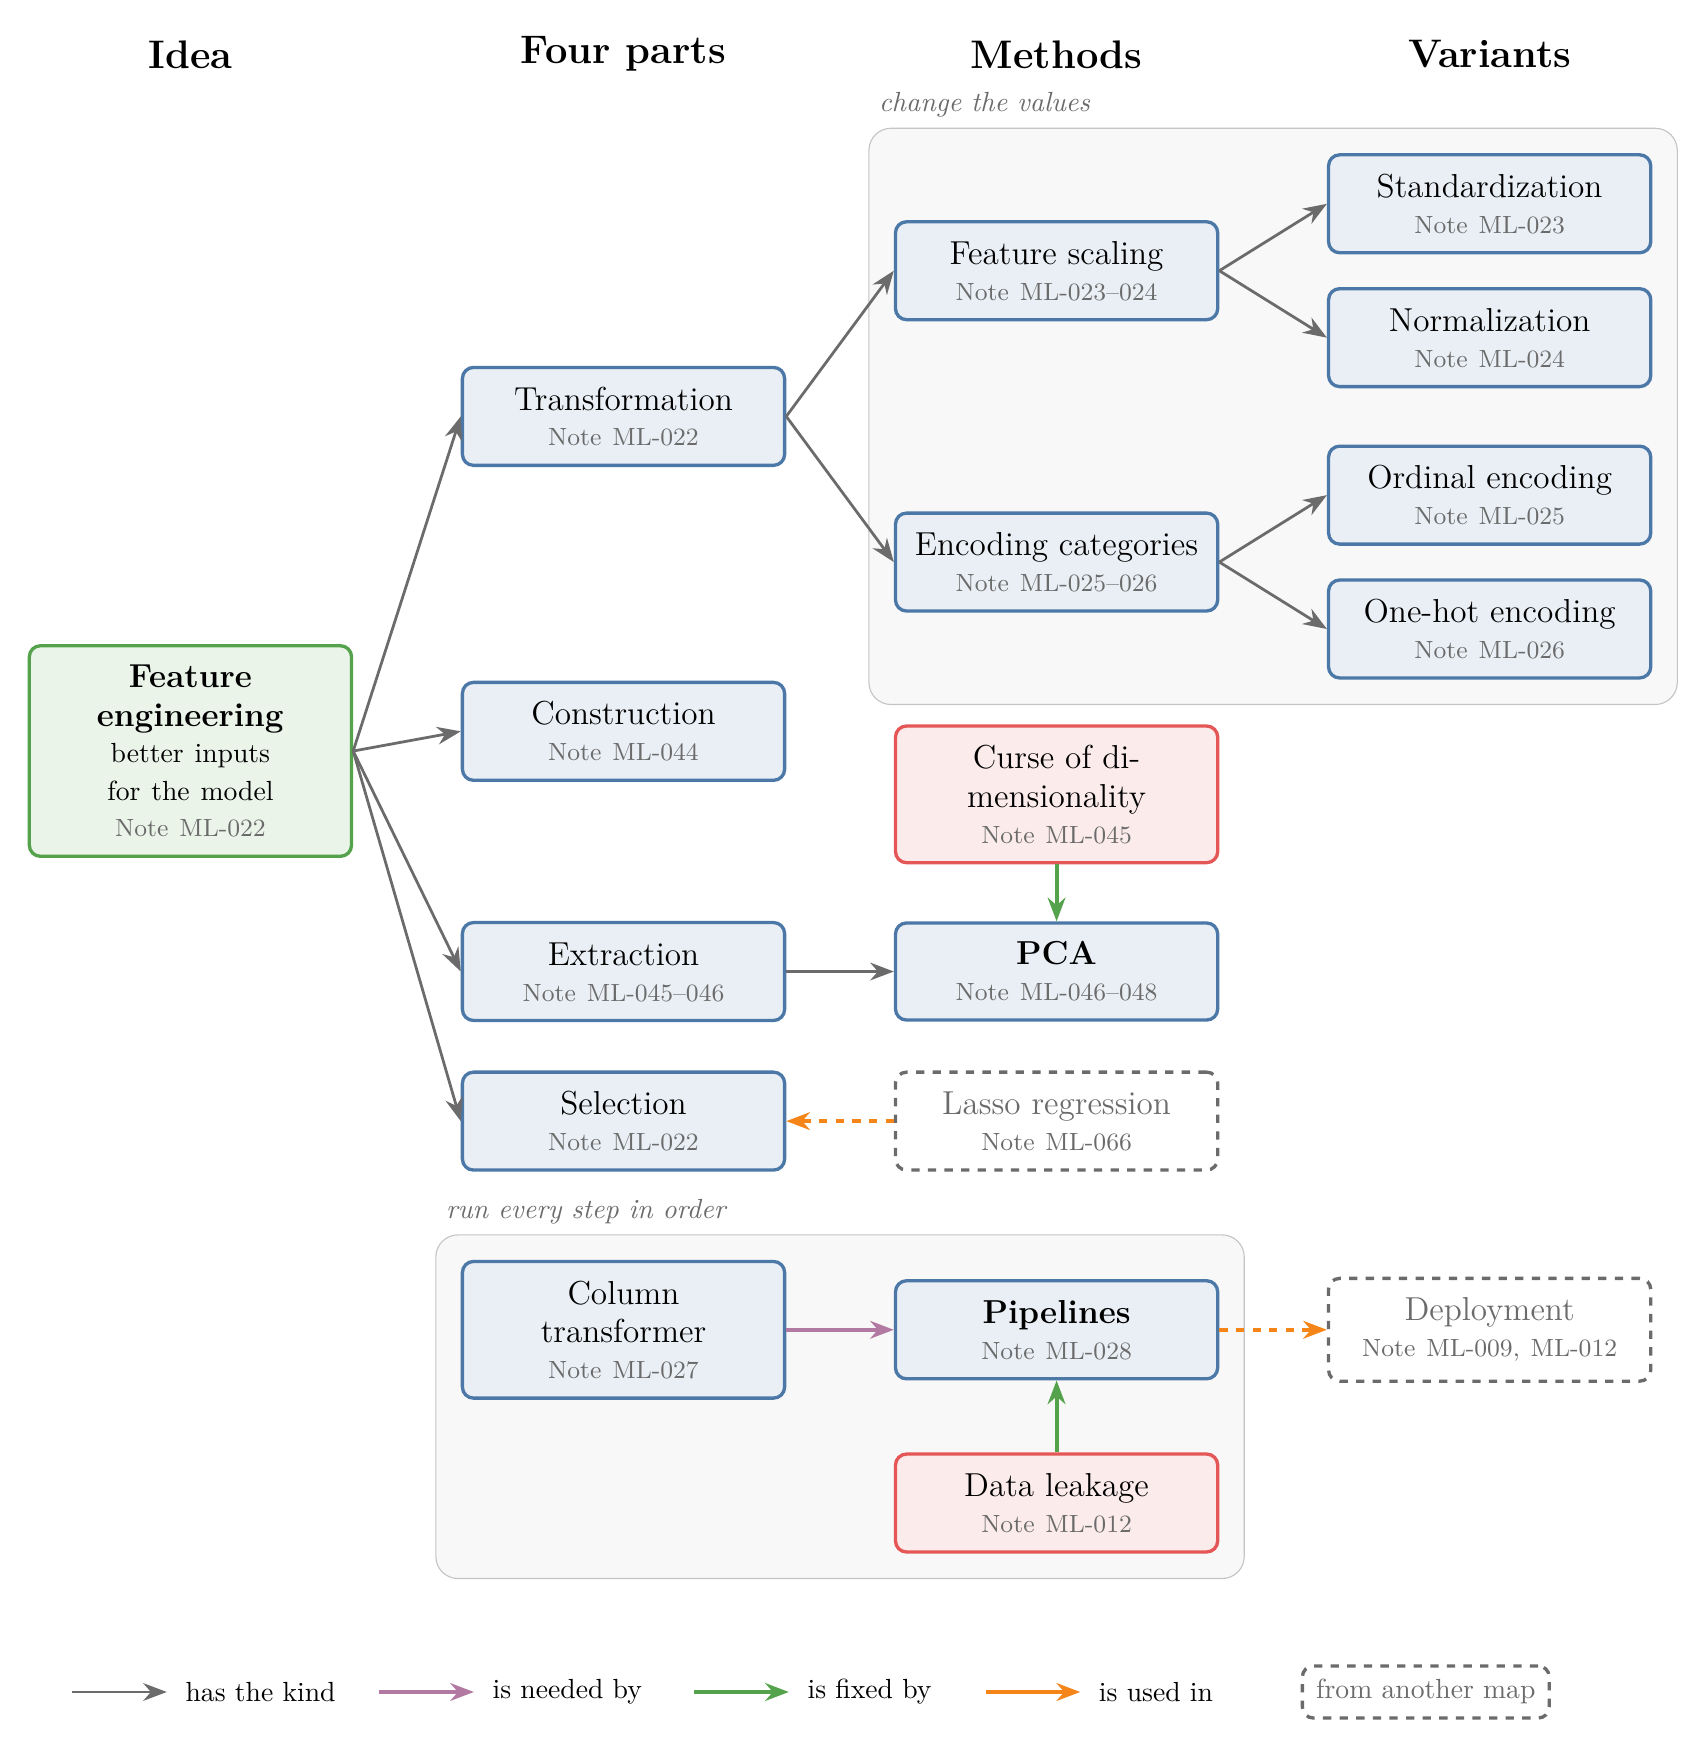
\begin{tikzpicture}[
    every node/.append style={font=\sffamily\large},
    con/.style={box=cblue, text width=3.6cm},
    prob/.style={box=cred, text width=3.6cm},
    prev/.style={draw=cgrey, dashed, rounded corners=4pt, align=center, inner sep=7pt, text=cgrey, text width=3.6cm, minimum height=1.1cm},
    group/.style={draw=cgrey!40, fill=cgrey!5, rounded corners=8pt, inner sep=9pt},
    gname/.style={font=\sffamily\normalsize\itshape, text=cgrey, anchor=south west},
    kindof/.style={arrow, draw=cgrey, line width=1pt},
    needs/.style={arrow, draw=cpurple},
    fixes/.style={arrow, draw=cgreen},
    usedin/.style={arrow, draw=corange},
  ]
  \newcommand{\nt}[1]{\\[-1pt]{\small\color{cgrey}Note #1}}
  \node[title] at (0,13.6)    {Idea};
  \node[title] at (5.5,13.6)  {Four parts};
  \node[title] at (11,13.6)   {Methods};
  \node[title] at (16.5,13.6) {Variants};

  % idea
  \node[box=cgreen, text width=3.6cm, minimum height=2.2cm] (fe) at (0,4.75) {\textbf{Feature}\\\textbf{engineering}\\[-1pt]{\normalsize better inputs for the model}\nt{ML-022}};

  % four parts
  \node[con] (tra) at (5.5,9.0) {Transformation\nt{ML-022}};
  \node[con] (con) at (5.5,5.0) {Construction\nt{ML-044}};
  \node[con] (ext) at (5.5,1.95) {Extraction\nt{ML-045--046}};
  \node[con] (sel) at (5.5,0.05) {Selection\nt{ML-022}};
  \foreach \p in {tra, con, ext, sel} \draw[kindof] (fe.east) -- (\p.west);

  % transformation: methods and variants
  \node[con] (sca) at (11,10.85)  {Feature scaling\nt{ML-023--024}};
  \node[con] (enc) at (11,7.15)   {Encoding categories\nt{ML-025--026}};
  \node[con] (std) at (16.5,11.7) {Standardization\nt{ML-023}};
  \node[con] (nor) at (16.5,10.0)  {Normalization\nt{ML-024}};
  \node[con] (ord) at (16.5,8.0)  {Ordinal encoding\nt{ML-025}};
  \node[con] (one) at (16.5,6.3)  {One-hot encoding\nt{ML-026}};
  \draw[kindof] (tra.east) -- (sca.west);
  \draw[kindof] (tra.east) -- (enc.west);
  \draw[kindof] (sca.east) -- (std.west);
  \draw[kindof] (sca.east) -- (nor.west);
  \draw[kindof] (enc.east) -- (ord.west);
  \draw[kindof] (enc.east) -- (one.west);

  % extraction and selection
  \node[prob] (cur) at (11,4.2) {Curse of dimensionality\nt{ML-045}};
  \node[con]  (pca) at (11,1.95) {\textbf{PCA}\nt{ML-046--048}};
  \draw[kindof] (ext) -- (pca);
  \draw[fixes] (cur) -- (pca);
  \node[prev] (las) at (11,0.05) {Lasso regression\nt{ML-066}};
  \draw[usedin, dashed] (las) -- (sel);

  % putting the steps together
  \node[con]  (ct)   at (5.5,-2.6) {Column transformer\nt{ML-027}};
  \node[con]  (pipe) at (11,-2.6)  {\textbf{Pipelines}\nt{ML-028}};
  \node[prob] (leak) at (11,-4.8)  {Data leakage\nt{ML-012}};
  \node[prev] (dep)  at (16.5,-2.6) {Deployment\nt{ML-009, ML-012}};
  \draw[needs] (ct) -- (pipe);
  \draw[fixes] (leak) -- (pipe);
  \draw[usedin, dashed] (pipe) -- (dep);

  \begin{scope}[on background layer]
    \node[group, fit=(sca) (std) (one)] (g1) {};
    \node[group, fit=(ct) (pipe) (leak)] (g2) {};
  \end{scope}
  \node[gname] at (g1.north west) {change the values};
  \node[gname] at (g2.north west) {run every step in order};

  % legend
  \begin{scope}[shift={(-1.5,-7.2)}, every node/.style={font=\sffamily, anchor=west}]
    \draw[kindof] (0,0) -- (1.2,0);   \node at (1.3,0) {has the kind};
    \draw[needs] (3.9,0) -- (5.1,0);  \node at (5.2,0) {is needed by};
    \draw[fixes] (7.9,0) -- (9.1,0);  \node at (9.2,0) {is fixed by};
    \draw[usedin] (11.6,0) -- (12.8,0); \node at (12.9,0) {is used in};
    \node[draw=cgrey, dashed, rounded corners=4pt, inner sep=5pt, text=cgrey, anchor=west] at (15.6,0) {from another map};
  \end{scope}
\end{tikzpicture}
\end{document}
